% !TEX root = ../thesis.tex

\chapter{Analytická časť}

\section{Vue}
Vue je progresívny frontendovy framework pre vytváranie použivateľských rozhraní (https://vuejs.org/v2/guide/). Zvolili sme ho pre účely tohto projektu, keďže je najjednoduchší na naučenie (v porovnaní s Reactom a Angularom). Štruktúra Vue kódu je veľmi podobná s klasickou HTML, CSS a Javascript syntaxou. Doplnená o pár direktív Vue (napríklad template tagy pre HTML časť).

Vue je v dnešnej dobe tretí najpopulárnejší framework z pomedzi 5 najväčších frontend frameworkov. 

\begin{figure}[!ht]
  \centering
  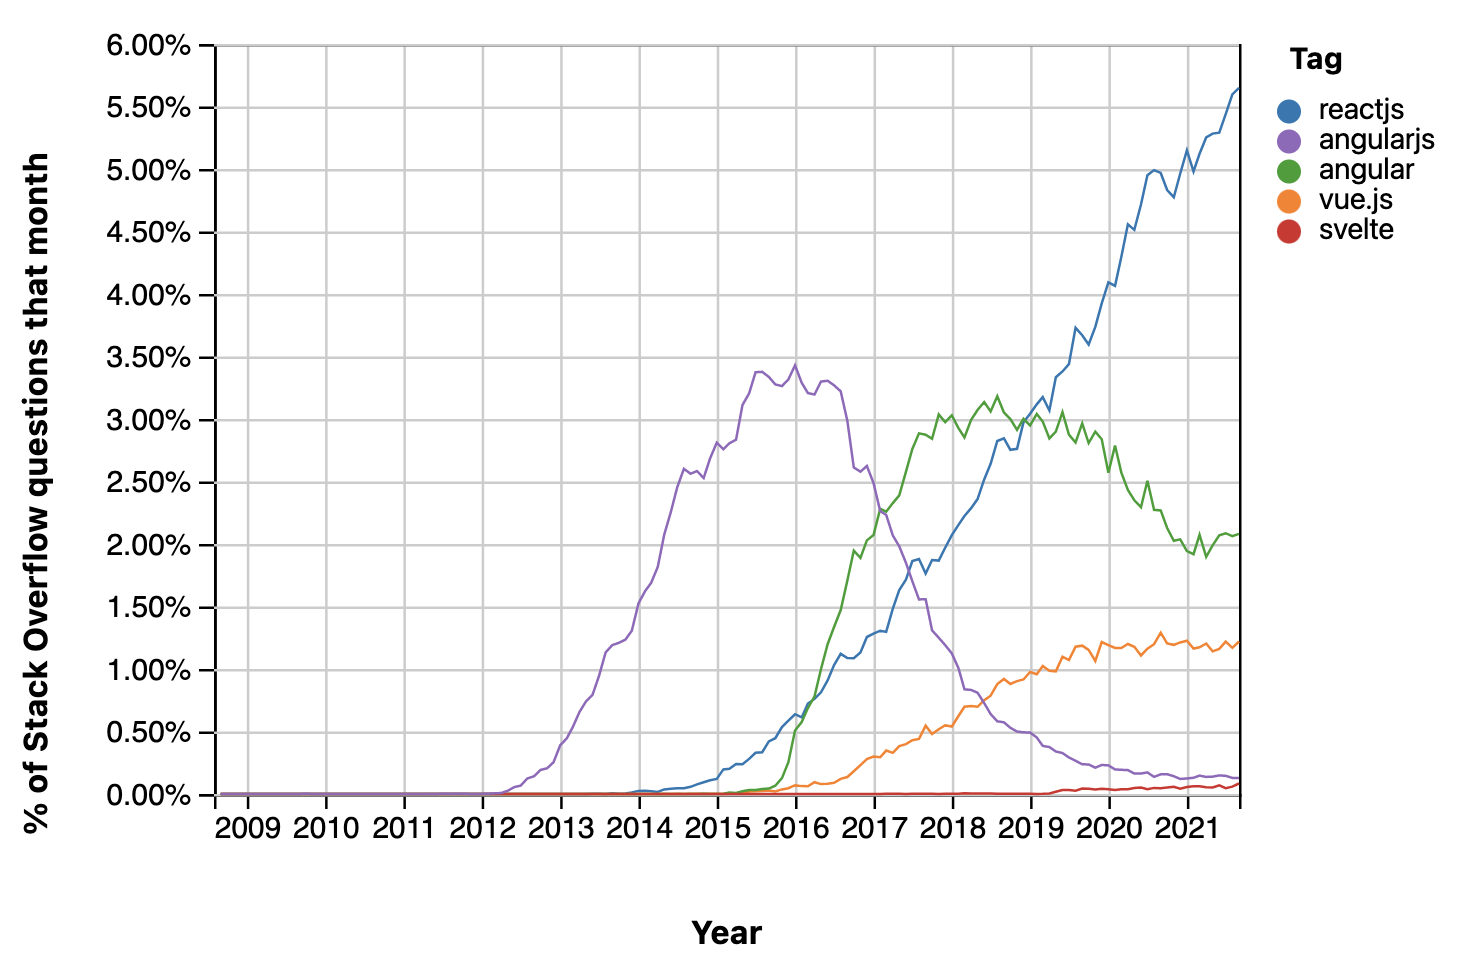
\includegraphics[width=.9\textwidth]{figures/frameworks.png}
  \caption{\LaTeX{} Vývoj popularity frameworkov v priebehu rokov \label{o:Vývoj popularity frameworkov v priebehu rokov}}
\end{figure}
https://gist.github.com/tkrotoff/b1caa4c3a185629299ec234d2314e190

Ak porovnáme tri najpoužívanejšie frameworky (React, Anuglar a Vue), tak si môžeme všimnúť rozdielne filozofiee, ktoré boli použité pri ich vytváraní. 

Angular si môžeme predstaviť ako veľkú dielňu. Nemusíme si zháňať ďalšie nástroje, pretože všetko čo potrebujeme sa v nej už nachádza. Naopak React by sme prirovnali ku kladivu. Jeho účelom je jediná vec a to je zrenderovať (vykresliť) UI. 

Vue je niečo medzi Angularom a Reactom. Aby sme zostali pri už použitej metafore tak Vue by bol pracovný kufrík, v ktorom máme uložené najviac podstatné nástroje, pre väčšinu projektov a ak potrebujeme nejaký viac špecifický nástroj, tak si ho môžeme do toho kufra pridať.

Okrem najprehľadnejšej syntaxi z pomedzi spomenutých frameworkov Vue taktiež rieši napríklad problém globálneho CSS z Reactu. Ktorý by sme pri väčšom projekte v Reacte museli riešiť napríklad pomcou BEM alebo Styled Components. Vue to rieši pomocou scooped CSS.

\subsection{Nuxt}
Nuxt je open source framework postavený na Vue. Nuxt sa nám snaží uľahčiť bežné problémy na ktoré narazíme pri vývoji appiek vo Vue. Jednou z nich je napríklad Automatický Router. Ak by sme chceli spravovať podstránky v klasickom Vue, museli by sme nastaviť súbor vue-router. Nuxt to rieši za nás a tento súbor generuje automaticky z jeho súborovej štruktúry. 

Základná inštalácia Nuxt projetku nám taktiež umožňuje pridať do projektu závislosti a vygeneruje nám súborovú štruktúru. Typesript pre statické typovanie, výber package manageru, UI knižnicu (Vuetify), Nuxt moduly (Axios, PWA, Content - git based headless CMS), Linting tool, Testing framework (Jest, Ava, WebdriverIO, Nightwatch), SSR/ SPA, Deployment Target (Server/ Static), Development tools,

\section{Critical Render Path}
Aby sme vedeli ako optimalizovať aplikáciu pre frontend. Bude nejlepšie ak sa najprv pozrieme na to akým spôsobom zobrazuje prehliadač dáta.

Critical Render Path je postup krokov ktoré, prehliadač vykonáva cez skompilovanie kódu po vykreslenie kontentu na obrazovke. 

Keď uvažujeme klient server model arhitektúru, môžme si CRP predstaviť následovným spôsobom. Client pošle request na server, a server mu pošle odpovedajúci súbor index.html. Prehliadač začne vytvárať Document object model, ktorý popisuje štruktúru stránky. Ako náhle sa v skripte objaví zmienka o CSS, prehliadač si ho vyžiada od servera. V momente keď dôjde CSS ku klientovi, prehliadač začne generovať CSS Object Model. Keď prehliadač uvidí v skripte scrip tag s Javscriptom, vypýta si JS od servera. Javascript na frontende začne modifikovať DOM. Po skompilovaní prehliadač vygeneruje render tree, čo je kompinácia DOM a CSSOM. Z neho prehliadač vydedukuje layout, pochopí kde má namaľov  ať content. Jedna z veci ktoré sme nespomenuli sú obrázky. Obrázky sa sťahujú špeciálnym spôsobom. Sú doťahované autmaticky čo na nich browser narazí pri čítaní index.html a sú sťahované na pozadí. Zobrazia sa na stránke hneď čo sú stiahnuté u klienta.